\chapter{Intelligente Tutorielle Systeme}
Intelligente Tutorielle Systeme\footnote{kurz ITS} sind eine um 1973 von Derek. H. Sleeman
und J.R. Hartley definierte Art von computergesteuerten Lernprogrammen.
Diese Art von Lernprogrammen waren der erste Ansatz, das in der Lerntheorie
ergründete Adaptive Lernen im softwaregestützten e-Learning zu etablieren,
um die Effizienz von Lernsoftware zu verbessern.

Intelligente Tutorielle Systeme erreichen ihre Adaptivität und Flexibilität durch
eine individuell an den Benutzer angepasste Art von Lernangeboten.
Das Verhalten während des Lernens, sowie die Leistungen während Lernüberprüfungen,
oder interaktiven Aufgaben, werden bewertet, um die Präsentation der Lerninhalte zu wählen.
Das bedeutet, dass ein Intelligentes Tutorielles System zu jeder Zeit versucht zu erkennen,
wie ausgeprägt das Wissen eines Anwenders in der jeweiligen Thematik ist, um die
zu vermittelnden Inhalte dementsprechend anzupassen, die dazu führen sollen ein
definiertes Lernziel zu erreichen.
So wird ein Anwender, der bisher keine Erfahrungen in einem Thema hat, nicht sofort
mit komplexen Sachverhalten konfrontiert, sondern langsam in die Thematik eingeführt,
bis er für die höheren Lernmaterialien bereit ist.


\section{Definition}
\glqq Intelligente tutorielle Systeme (ITS) sind adaptive Mediensysteme, die sich ähnlich
einem menschlichen Tutor an die kognitiven Prozesse des Lernenden anpassen
sollen, indem sie die Lernfortschritte und -defizite analysieren und dementsprechend
das Lernangebot generativ modifizieren sollen.\grqq{} \cite[S. 555]{issing2002information}

Die Intelligenz eines Intelligenten Tutoriellen Systems besteht dementsprechend
in der Adaption der Lehrinhalte an den Wissensstand des jeweiligen Benutzers.
Ein ITS versucht, vergleichbar mit einem menschlichen Lehrer, einen flexiblen und adaptiven
Dialog mit dem Lernenden zu führen, indem es den Unterricht den Merkmalen und Fortschritten
des Benutzers anpasst.

Signifikant für ein Intelligentes Tutorielles System sind hierbei folgende drei Hauptmerkmale:

\begin{description}
	\item[Adaptivität]
  Adaptivität beschreibt die Fähigkeit des Systems, sich selbstständig an den
  jeweiligen Benutzer anzupassen. Dies geschieht durch die Auswertung von
  Informationen über zur Verfügung stehenden Lerninhalten, Bewertung des Lernenden, sowie
  der Anwendung von definierten pädagogischen Strategien.
  Vergleichbar ist dies mit einer typischen Situation, mit der sich ein
  menschlicher Lehrer bei der Gestaltung seines Unterrichts konfrontiert sieht.
  Einem Lehrer ist es nicht möglich, während der Vorbereitung seines Unterrichts
  zu wissen, welche Strategien er später im Unterricht benötigen wird, um
  das zu übermittelnde Wissen optimal zu erklären. Er ist dazu gezwungen sich
  im Laufe des Unterrichts dynamisch an die Situation anzupassen.

	\item[Flexibilität]
  Die Flexibilität des Systems bezieht sich auf die Fähigkeit, die Darstellung
  der Lerninhalte zu verändern. Diese Fähigkeit wird durch die getrennte
  Realisierung der Wissensbasis und der tutoriellen Komponente ermöglicht.
  Diese beiden Begriffe werden im Laufe dieser Ausarbeitung näher erläutert.

	\item[Diagnosefähigkeit]
  Die Diagnosefähigkeit ist ein weiterer Kernaspekt eines Intelligenten Tutoriellen Systems.
  Sie beschreibt die Fähigkeit, den aktuellen Wissensstand, sowie weitere Kriterien
  des Lernenden zu analysieren, um so Rückschlüsse über seine themen- und lernspezifische
  Kompetenz zu bewerten.
  Auf diese Art und Weise versucht ein Intelligentes Tutorielles System ein Modell des
  Lernenden abzuleiten, um darauf basierend eine passende individuelle Lehrstrategie
  für den Lernenden zu entwickeln.
  Ohne diese Fähigkeit wäre ein ITS nicht dazu in der Lage,
  seine Inhalte auf eine sinnvolle Art und Weise individuell an einen Lerner anzupassen.
\end{description}

Wichtig ist, dass der Lernablauf weiterhin benutzergesteuert ist. Der Benutzer steuert
selbst, in welcher Geschwindigkeit er seinen Lernprozess gestaltet.
Das Intelligente Tutorielle System bietet dem Benutzer hierbei jedoch nur zu
der Bewertung seines Wissensstand passende Lernmaterialen an, um mit dem Lernen
fortzufahren. So soll gewährleistet werden, dass er Lernende das Lernziel auf einem
für ihn optimalen Weg erreicht.

\section{Unterschiede zu klassischen tutoriellen Systemen}
Um zu verstehen, wodurch sich Intelligente Tutorielle Systeme von den früheren
klassischen Tutoriellen Systemen unterscheiden, muss zunächst die Funktionsweise
von klassischen Tutoriellen Systemen erörtert werden.

Bei klassischen Tutoriellen Systemen handelt es sich ebenfalls um Lernsoftware,
die einem Lernenden auf (multi)mediale Art und Weise Lehrstoff präsentiert, um ein
definiertes Lernziel zu erreichen. Es handelt sich hierbei jedoch nicht um reine
Präsentationssysteme.

\begin{figure}[!htb]
	\centering
	\begin{tikzpicture}[
				part/.style={rectangle, minimum width=4cm, minimum height=2cm, very thick, draw=black, font=\itshape}
				]
		\node (start) [part] {Programmstart};
		\node (presentation) [part, right=of start] {Lehrstoffpräsentation};
		\node (question) [part, right=of presentation] {Fragestellung};
    \node (end) [part, below=of start] {Programmende};
    \node (feedback) [part, below=of presentation, right=of end] {Feedback};
		\node (analyze) [part, below=of question, right=of feedback] {Analyse der Antwort};


		\draw [->] (start) -- (presentation);
		\draw [->] (presentation) -- (question);
		\draw [->] (question) -- (analyze);
		\draw [->] (analyze) -- (feedback);
		\draw [->] (feedback) -- (presentation);
		\draw [->] (feedback) -- (end);
	\end{tikzpicture}

	\caption{Prinzip eines klassischen tutoriellen Systems}
\end{figure}

In der Abbildung ist erkennbar, dass tutorielle Systeme zusätzlich zur
reinen Präsentation der Lehrinhalte, zwischendurch einige Fragen an den Lernenden stellen.
Die Antworten auf diese Fragen, die der Lernüberprüfung dienen, beeinflussen den weiteren
Verlauf des Lernkurses. Wichtig hierbei ist, dass lediglich der Ablauf des Lernkurses
beeinflusst wird. So wird ein Lehrinhalt bei unzureichendem Ergebnis in der Leistungsüberprüfung
solange wiederholt, bis der Lernende dazu in der Lage ist, die Fragestellung korrekt zu beantworten.
In einem tutoriellen System erhält der Lernende üblicherweise sofort Feedback auf
seine erbrachte Leistung.
Bei einer falschen Antwort kann das beispielsweise die Angabe der korrekten Lösung,
oder ein Hinweis auf den richtigen Lösungsweg sein. Dieses Feedback simuliert
hierbei die Rolle eines Tutors.

Klassische tutorielle Systeme lassen sich in der Regel dem behavioristischem Lernparadigma
zuordnen. Die Software repräsentiert eine absolute Lehrautorität, die dem Lernenden
Wissen präsentiert. Die Bewertung von Antworten beschränkt sich auf falsch oder richtig.

Ein einfaches Beispiel für ein klassisches tutorielles System ist das Lernen für
die theoretische Fahrschulprüfung mit Hilfe einer Handy-Applikation. Klassisch werden
hierbei die aus den offiziellen Fragebögen bekannten Fragen repetetiv präsentiert,
und der Benutzer dazu aufgefordert, eine Antwort auszuwählen.

\begin{figure}[!htb]
	\centering
    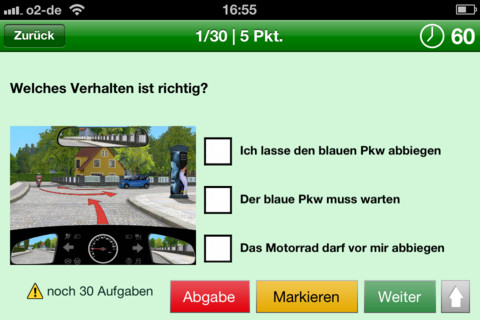
\includegraphics[width=0.7\textwidth]{bilder/fahrschule_app.jpg} %70% der Textbreite
	\caption{Beispielbild der Pocket Fahrschule Handy-Applikation}
\end{figure}

Tut er dies, wird ihm unmittelbar nach der Eingabe der Antwort vermittelt,
ob diese richtig oder falsch war.
Bei komplexeren Fragestellungen wird, je nach Applikation, zusätzlich erläutert warum
die korrekte Lösung korrekt ist.
Nach diesem Verfahren wird fortgefahren, bis der Lernende alle vorhandenen Fragen
korrekt beantwortet hat.

Intelligente Tutorielle Systeme versuchen darüber hinaus die Erkenntnisse neuerer Lernparadigmen,
wie zum Beispiel dem Kognitivismus zu berücksichtigen.
Im Gegensatz zu einem klassischen System kann ein ITS individuelle Kritik an einen Lernenden
formulieren.

\begin{figure}[!htb]
	\centering

	\begin{tikzpicture}[->,>=stealth', node distance=2cm,
                    semithick]
			\tikzstyle{comp2} = [fill=yellow, draw, rectangle, rounded corners, minimum height=0.8cm]
			\tikzstyle{comp3} = [fill=black, text=white, draw, rectangle, rounded corners, minimum height=0.8cm]
			\tikzstyle{comp1} = [draw, rectangle, rounded corners, minimum height=0.8cm]


			\node[comp2] (A)                    {Erstelle ein Problem};
			\node[comp2] 				 (I) [above right of=A]       {Lehrinhalt / Curriculum};
			\node[comp2]         (B) [below of=A] {Präsentiere das Problem};
			\node[comp2]         (E) [below of=B] {Vergleiche die Lösungen};
			\node[comp1]         (C) [below right of=E] {Lösung};
			\node[comp3]         (H) [right of=C] {Student};
			\node[comp1]         (D) [below left of=E] {Musterlösung};
			\node[comp2]         (F) [below right of=D] {Aktualisiere Wissenskenntnis vom Studenten};
			\node[comp2]         (G) [below of=F] {Gebe Feedback};

			\path (I) edge              node[right] {basierend auf} (A)
						(A) edge              (B)
						(B) edge              (E)
						(H) edge [bend right]  node[above] {gibt} (C)
						(D) edge              (E)
						(C) edge              (E)
						(E) edge              (F)
						(F) edge              (G)
						(G) edge [bend angle=105, bend left]              (A)
			%% 					edge              node {1,1,R} (C)
			%% (B) edge [loop above] node {1,1,L} (B)
			%% 		edge              node {0,1,L} (C)
			%% (C) edge              node {0,1,L} (D)
			%% 		edge [bend left]  node {1,0,R} (E)
			%% (D) edge [loop below] node {1,1,R} (D)
			%% 		edge              node {0,1,R} (A)
			%% (E) edge [bend left]  node {1,0,R} (A);
			;
			\end{tikzpicture}
	\caption{Lernablauf in einem Intelligenten Tutoriellen System}
	\label{fig:its_flow}
\end{figure}

Abbildung~\ref{fig:its_flow} zeigt den typischen Ablauf des Lernverfahrens in einem Intelligenten Tutoriellen Systems.
Prinzipiell wird von dem System auf Basis des gegebenen Lehrstoffes und dem aktuellen Wissensstand
des Lernenden ein Problem als Aufgabe erstellt und präsentiert. Der vom Lernenden gegebene Lösungsvorschlag
wird mit der vorhandenen Musterlösung verglichen und bewertet. Auf Basis der abgegebenen Lösung
wird der aktuelle Wissensstand über den Lernenden aktualisiert und gegebenenfalls Feedback gegeben.
Anschließend beginnt der Lernablauf wieder von vorne, bis der gesamte Lehrstoff vermittelt wurde.

Der präsentierte Lehrinhalt ist nicht statisch, also in jedem Fall gleich, sondern
angepasst an die individuellen Bedürfnisse eines Lernenden.
Auf diese Weise sind ITS dazu in der Lage auch komplexere Sachverhalte zu vermitteln.

\section{Struktur}
Wie jede Software entsprechen auch Intelligente Tutorielle Systeme einer klar definierten Architektur.
In der Abbildung ist zu sehen, dass ein Intelligentes Tutorielles System aus vier
Hauptkomponenten besteht, die getrennt voneinander implementiert werden.

\begin{figure}[!htb]
	\centering
    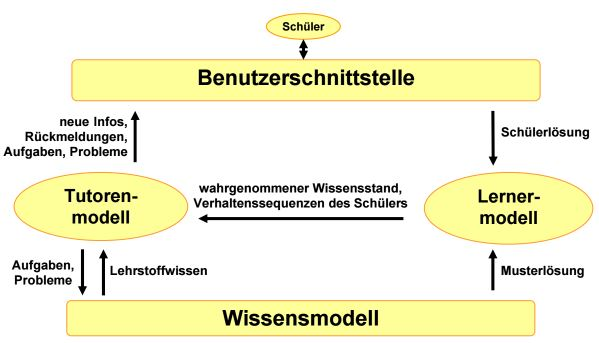
\includegraphics[width=0.7\textwidth]{bilder/its_structure.jpg} %70% der Textbreite
	\caption{Struktur eines Intelligenten Tutoriellen Systems}
\end{figure}

%% TODO: das Schaubild mit tikz nachstellen wäre schöner.
%%\begin{figure}
%%\centering
%%
%%	\begin{tikzpicture}[node distance=2.2cm]
%%
%%		\tikzstyle{comp1} = [draw, ellipse, rounded corners, minimum height=1cm, minimum width=4cm, fill=gray!50]
%%		\tikzstyle{comp2} = [draw, rectangle, rounded corners, minimum height=1cm, minimum width=4cm]
%%		\tikzstyle{comp3} = [draw, ellipse, minimum height=1cm, minimum width=4cm, fill=gray!10, text centered]
%%
%%		\tikzstyle{arrow} = [thick,->,>=stealth]
%%
%%		%%% NODES %%%
%%		\node (tutand)     [comp1]                 {Lernender};
%%		\node (ui)     		 [comp2, below of=tutand, minimum width=10cm]                 {Benutzerschnittstelle};
%%		\coordinate[below of=ui] (c);
%%
%%		\node (tutor)         [comp3, left of=c]      {Tutorenmodell};
%%		\node (learn)        [comp3, right of=c]     {Lernermodell};
%%		\node (knowledge)       [comp2, below of=c,minimum width=10cm]     {Wissensmodell};
%%
%%		%%% ARROWS %%%
%%		\draw [arrow] (tutand) -- (ui);
%%
%%		\draw [arrow] (ui) -- (tutand);
%%		\draw [arrow] ([yshift=-0.5cm, xshift=-2.8cm]ui.east) -- (learn);
%%
%%		\draw [arrow] (learn) -- (tutor) node [midway, fill=white, text width=3cm] {wahrgenommener Wissensstand,\linebreak Verhaltenssequenzen des Lernenden};
%%
%%		\draw [arrow] (tutor) -- (knowledge);
%%
%%		\draw [arrow] (knowledge) -- (tutor);
%%		\draw [arrow] (knowledge) -- (learn);
%%	\end{tikzpicture}
%%	\caption{Struktur eines Intelligenten Tutoriellen Systems}
%%\end{figure}

Die Kanten des Graphen, unter hinzunahme ihrer Beschriftungen, beschreiben die Art der
Kommunikation zwischen den einzelnen Komponenten.
Man sieht, dass die einzige Kommunikation zwischen dem Lernenden und dem System über die
bereitgestellte Benutzerschnittstelle statt findet. Ein beispielhafter Ablauf könnte sein:

Der Schüler löst eine Aufgabe. Über die Benutzerschnittstelle wird dessen Lösung
an das Lernermodell weitergeleitet. Das Lernermodell erhält gleichermaßen vom Wissensmodell
die Musterlösung der zu lösenden Aufgabe. An dieser Stelle werden die beiden Lösungsansätze
verglichen, um mit Hilfe dieses Vergleichs den Wissensstand und die Verhaltensweisen
des Lernenden abzuleiten. Das Ergebnis dieser Analyse wird dem Tutorenmodell mitgeteilt, welches
auf Basis der Analyse geeignete pädagogische Lernstrategien für den Lernenden einschlagen kann,
und ihm entsprechend seiner Bedürfnisse Feedback liefern kann. Dieses wird dem Lernenden
über die Benutzerschnittstelle kommuniziert. Im weiteren Verlauf der Ausarbeitung
wird nun genauer auf die einzelnen Komponenten eingegangen.

\subsection{Das Wissensmodell}
%% - auch Expertenmodell
%% - bildet Wissensbasis des Lernsystems.
%% - Ansammlung von Kenntnissen, Erfahrungen, Methoden und Allgemeinwissen.
%% - Verkörpert drei verschiedene Wissenskategorien:
Das Wissensmodell wird häufig auch das Expertenmodul genannt. Es repräsentiert den vollständigen
Wissensstand über die zu lehrende Thematik des Intelligenten Tutoriellen Systems.
Das Wissensmodell ist zwingend notwendig, damit das System im Lernermodell dazu in der Lage ist,
den aktuellen Wissensstand des Lerners zu analysieren.
Es besteht aus einer statischen Ansammlung von Kenntnissen, Erfahrungen, Methoden und Allgemeinwissen.

\subsubsection{Wissenskategorien}
Das Wissen wird hierbei in drei unterschiedliche Kategorien eingeteilt:

\begin{description}
	%% -- Deklaratives Wissen (Faktenwissen, "Was-Wissen")
	%% --- "Vokabelwissen" -> Definition von notwendigen Begriffen, etc. (z.B. im
	%% Kontext Mathe - was ist eine Wurzel, was ist Addieren...)
	\item[Deklaratives Wissen]
  Das deklarative Wissen repräsentiert \glqq Wissen-Was\grqq{} -Wissen, oder auch Faktenwissen.
	Es handelt sich hierbei um Sachverhalte, die
	auswendig gelernt werden können. Beispiele hierfür wären die Anzahl der Wirbel einer menschlichen Wirbelsäule,
	oder das Faktum, dass \(1+1=2\) ist.
	Dieses Wissen kann grundsätzlich durch verschiedene Formen repräsentiert werden.
	So kann es beispielsweise in Textform vermittelt werden, oder durch Schaubilder,
	die diese Fakten eindeutig erläutern.

	%% -- Prozedulares Wissen (praktisches Wissen, "Wie-Wissen")
	%% --- Beinhaltet Regeln, mit deren Hilfe sich Problemstellungen lösen lassen
	%% --- Regelwissen (Schema, nach dem ich vorgehen muss zum Addieren ...)
	%% --- Basis von Prozedularem Wissen ist stets deklaratives Wissen
	%% ---- ist also: wie setze ich deklaratives Wissen zusammen, um eine Problemstellung zu lösen.
	\item[Prozedurales Wissen]
  Prozedurales Wissen wird auch praktisches Wissen oder \glqq Wissen-Wie\grqq{} -Wissen genannt.
	Es handelt sich hierbei um Erkenntnisse, auf welche Art und Weise man bekanntes Wissen anwenden kann,
	um bestimmte Problemstellungen zu lösen.
	Gemeint sind hiermit bestimmte Zusammensetzung von Regeln, oder auch Schemata, mit Hilfe deren man
	ein gewünschtes Ergebnis erreicht werden kann.
	Ein klassisches Beispiel für diese Art von Wissen ist die schriftliche Multiplikation.
	Man nehme als Beispiel die Lösung der Problemstellung \(15*25=?\).
	Dieses Problem kann schematisch in kleineren Schritten gelöst werden, und zwar aus der Addition der
	zwei Teilprodukte \(15*20\) und \(15*5\).
	Diese herangehensweise ist ein Beispiel für prozedurales Wissen, da es einen Satz von Regeln beschreibt,
	mit Hilfe deren ich dazu in der Lage bin, schriftlich zu multiplizieren.
	Wichtig hierbei ist, dass die Basis von prozeduralem Wissen immer deklaratives Wissen ist.
	Prozedulares Wissen vermittelt stets Regeln, die deklaratives Wissen, möglicherweise verknüpft, verwenden,
	um komplexe Problemstellungen zu lösen.

	%% -- Heuristisches Wissen (Erfahrungswissen)
	%% --- Beinhaltet Erfahrungswerte von Experten, bspw. um Bekannte Fehler zu erkennen und daraufhin
	%% --- bekannte Tipps geben zu können.
	%% --- Handlungsempfehlungen
	%% --- Dient der Unterstützung zur Findung einer richtigen Herangehensweise an ein Problem
	\item[Heuristisches Wissen]
  Das heuristische Wissen beinhaltete im wesentlichen Erfahrungswerte von Lehrenden.
	Es wird daher auch häufig Erfahrungswissen genannt.
	Es handelt sich hierbei um typische Handlungsempfehlungen, die einem Lernenden
	dabei unterstützen können, die richtige Herangehensweise an eine Problemstellung zu finden.
	Im wesentlichen sind es Tipps, die sich im Laufe der Zeit in der Regel als hilfreich erwiesen haben.
\end{description}

%% - Kann auf zwei versch. Arten repräsentiert werden.
%% -- Black Box Modell
%% --- Vorgehensweisen vom Programm sind verborgen
%% --- Nur Ergebnisse von Lösungen sind einsehbar
%% --- Bildet keine menschliche Intelligenz nach, daher wird Lösungsweg verschleiert.
%% --- Kann kompliziertere Fragestellungen schneller berechnen, da kein Wert auf Nachvollziehbarkeit gelegt wird.
%% -- Glass Box Modell
%% --- Jeder Einzelschritt ist einsehbar.
%% --- Erhebt Anspruch menschen vergleichbare Methoden zur Problemlösung anzuwenden
%% --- Vollständiger Lösungsweg ist jederzeit sichtbar, Lernender kann interaktiv Fragen Stellen
%% --- Modell kann Lernenden zu jeder Zeit Schritt für Schritt helfen.
%% - Formell harte Abgrenzung, oft werden die Formen vermischt.
\subsubsection{Repräsentationsmöglichkeiten}
Die Repräsentationsmöglichkeiten des Wissensmodells werden im wesentlichen in zwei verschiedene
Modelle eingeteilt.

Zum einen gibt es das \glqq Black-Box-Modell\grqq .
In diesem Modell sind die Vorgehensweisen des Programms, mit deren Hilfe es dazu
in der Lage ist, eine Problemstellung zu lösen, verborgen. Dem Lernenden sind lediglich
die Ergebnisse der Lösungen einsehbar. Dieses Modell hat keine Ambitionen, menschliche
Intelligenz nachzustellen. Der Vorteil hiervon ist die leichtere Umsetzung zur Lösung
auch komplizierter Sachverhalte, da es nicht notwendig ist, darauf zu achten, dass die
Lösungswege für einen Menschen nachvollziehbar sind.

Das alternative Modell ist das \glqq Glass-Box-Modell\grqq .
Dieses Modell erhebt den Anspruch, menschenähnliche Denkweisen zum Lösen von
Problemstellungen nachzubilden. Auf diese Weise ist es dem Lernenden zu jeder Zeit der
Problembearbeitung möglich, mit dem System zu interagieren. Das System ist nun in der Lage
dem Lernenden Schritt für Schritt an die richtige Lösung heranzuführen.


%% - Wissen meist in Form von semantischen Netzen modelliert
%% -- Wie ein Graph/Baum
%% -- Knoten repräsentieren Wissenseinheiten
%% -- Kanten repräsentieren Verknüpfungen zwischen Wissen
%% -- Üblicherweise in einer Hierarchie
%% --- Wissen von einer Ebene ist Voraussetzung, für verbundenes Wissen in nächster Ebene.
\subsubsection{Das semantische Netz}
Strukturell wird Wissen im Allgemeinen in der Regel in Form von semantischen Netzen modelliert.
Die Idee von semantischen Netzen geht zurück auf die Forschungen von Ross Quillian aus dem Jahre 1967,
in denen er semantische Netze als Darstellung von menschlichem Wissen diskutierte.

Ein semantisches Netz kann man sich als Graphen vorstellen. Die Knoten des Graphen repräsentieren
hierbei einzelne atomare Wissenseinheiten. Kanten, mit denen zwei Knoten verbunden werden können,
zeigen, dass diese beiden Wissenseinheiten miteinander verknüpft sind. Sie stellen also die Relationen zwischen
den einzelnen Wissenseinheiten dar.\cite[S.5ff]{reichenberger2010}

Eine mögliche Form einer Relation, die auch häufig in semantischen Netzen für ein ITS verwendet wird,
ist eine Voraussetzung. Solch eine Relation würde ausdrücken, dass eine Wissenseinheit zwingend notwendig ist,
um eine andere Wissenseinheit zu verstehen. In diesem Fall würde es sich bei dem semantischen Netz um einen gerichteten Graphen handeln.

\begin{figure}[!htb]
	\centering

	\begin{tikzpicture}[->,>=stealth', node distance=2cm and 2cm,
                    semithick]
			\tikzstyle{comp2} = [fill=yellow, draw, rectangle, rounded corners, minimum height=0.8cm]

			\node[comp2]	(A)                    	{Addition};
			\node[comp2]  (B) [right=of A] 				{Subtraktion};
			\node[comp2]  (C) [above=of A] 				{schriftl. Addition};
			\node[comp2]  (D) [above of=B, right=of C] 	{schriftl. Subtraktion};
			\node[comp2]  (E) [above of=A, left=of C] 	{Multiplikation};
			\node[comp2]  (F) [above of=C] 	{Division};
			\node[comp2]  (G) [above of=E] 	{schriftl. Multiplikation};

			\path (A) edge              (B)
						(A) edge              (C)
						(A) edge              (E)
						(B) edge              (D)
						(C) edge              (D)
						(E) edge              (G)
						(E) edge              (F)
			;
			\end{tikzpicture}
	\caption{Theoretisches Beispiel für ein semantisches Netzwerk mit Abhhängigkeitsrelationen}
	\label{fig:semantic_net}
\end{figure}

Abbildung~\ref{fig:semantic_net} zeigt vereinfacht und beispielhaft ein semantisches Netzwerk mit Abhängigkeitsrelationen
für einen Teilbereich der Mathematik.
Eine solche Darstellung des Wissens ermöglicht es dem ITS, herauszufinden welche Wissenseinheit
geeignet für den aktuellen Wissensstand des Lernenden ist, und welche er noch nicht verarbeiten kann.

\subsection{Das Lernermodell / Das Tutandenmodell}
%% - enthält zu jedem Zeitpunkt aktuell bekannten Wissensstand.
%% -- aufgeteilt in:
%% --- Was weiß der Student? (Know that) --> deklaratives Wissen
%% --- Was kann der Student? (Know how) --> prozedurales Wissen
%% --- Was hat er bisher gemacht? (Historie)
Das Lernermodell stellt zu jedem Zeitpunkt den aktuell bekannten Wissensstand des Lernenden dar.
Jede Aktion des Lerners führt zu einer neuen Bewertung seines Wissens. Das Lernermodell ist daher stark dynamisch.
Das ist notwendig damit das Intelligente Tutorielle System zu jeder Zeit dazu in der Lage ist, sich voraussichtlich optimal
auf den Lernenden einzustellen.
Passens zum Wissensmodell ist auch das Wissen des Lerners im Lernermodell in zwei Kategorien aufgeteilt.
Es handelt sich hierbei um deklaratives und prozedurales Wissen. Bei beidem handelt es sich um Wissen, dass
in der Form auch im Wissensmodell bekannt ist.

%% - enthält außerdem Informationen darüber, was für ein Lerntyp
%% - Lernender wahrscheinlich ist (individuelle Aussage über Lernenden)
%% -- Wissen durch Monitorung der Historie/Ergebnisse
%% -- oder durch Fragebögen
Zusätzlich zum reinen Wissen enthält das Lernermodell auch eine
Historie aller Aktionen, die der Lerner vorgenommen hat. Über die Historie lassen sich Voraussagen über Vorlieben, Stärken
und Schwächen des Lernenden treffen. Dies ist notwendig, um den Lernenden einem Lernstereotypen zuzuordnen.
Solches Wissen lässt sich ebenfalls über eine zusätzliche Befragung des Lerners aneignen.

%% - typisches Lernerwissensmodell ist das Overlay-Modell.
%% -- Overlay-Modell (Untermenge)
%% --- Vergleicht jedes Wissenselement des Lernthemas mit Wissensstand des Lerners.
%% --- Wissen des Lernenden ist Teilmenge von Systemwissen.
%% --- Streng genommen wird notiert, ob Lernender Wissenselement beherrscht oder nicht
%% --- in der Praxis zu streng, es wird bewertet "wie gut" der Lernende etwas kann.
%% --- Fehler werden als unvollständiges Wissen betrachtet
Eine typische Form ein Lernermodell darzustellen ist das Overlay-Modell.
Bei dem Overlay-Modell wird das Wissen des Lernenden stets als Teilmenge des Systemwissens betrachtet.
Jedes bekannte Wissenselement der Lerndomäne wird mit dem aktuellen Wissensstand des Lerners verglichen.
Streng genommen wird hierbei lediglich notiert, ob der Lernende dieses Wissenselement optimal beherrscht, oder gar nicht.
Diese strenge Trennung ist in der Praxis jedoch zu stark, weswegen typischerweise eine Bewertung jeder Wissenseinheit vorgenommen wird.
So wird bewertet, zu welchem Grad der Lernende das entsprechende Wissensteil beherrscht.
Im Overlay-Modell werden Fehler stets als unvollständiges Wissen betrachtet.

%% - Overlay Modell nur in der Lage zu sagen DASS Lernender Wissen nicht hat.
%% - Vorhandenes, aber falsches Wissen ist nicht abbildbar.
%% - kann auch sein, dass Wissen korrekt vorhanden ist, aber falsch eingesetzt wird.
%% - daher zusätzlich zum Overlay-Modell Fehlerbibliothek.
Diese Art von Lernerwissensmodell ist in reiner Form lediglich dazu in der Lage, zu erkennen,
dass ein Lernender bestimmtes Wissen nicht besitzt.
Bereits vorhandenes, aber eventuell leicht verfälschtes Wissen ist auf diese Art und Weise nicht abbildbar.
Denkbar ist auch, dass der Lernende bestimmtes Wissen bereits besitzt, es jedoch lediglich falsch anwendet.
Um diese Defizite auszugleichen, erweitert man das Overlay-Modell häufig noch um eine Fehlerbibliothek.

%% -- sammelt typische Fehler und Missverständnisse von Lernern
%% -- hilft dem ITS dem Lernenden schneller entsprechende Tipps zu geben
%% --- Beispiel: schriftl. Addieren (vergessen vom übertrag)
%% -- ist häufig sehr groß und unterschiedlich
%% -- ist unmöglich, alle Fehler vorherzusagen.
Eine Fehlerbibliothek besteht aus typischen Fehlern und Missverständnissen von Lernen.
Mit Hilfe der Fehlerbibliothek ist es dem Tutorenmodell später möglich, eine bestimmte Art von
Fehlern zu erkennen, und durch entsprechende Hinweise zu korrigieren.
Ein Beispiel hierfür wäre ein vergessener Übertrag beim schriftlichen Addieren.
Es handelt sich um einen typischen Fehler, der jedoch nicht bedeutet, dass der Lernende nicht dazu in der Lage ist
zu addieren. Er vergisst lediglich einen Schritt.
Eine Fehlerbibliothek ist häufig sehr groß. Es ist auch unmöglich zum Zeitpunkt des Anlegens der Fehlerbibliothek
alle möglichen Fehler zu berücksichtigen oder vorherzusagen. Daher ist eine Fehlerbibliothek stets unvollständig.

\subsection{Das Tutorenmodell / Die Didaktikkomponente}
%% - simuliert das Verhalten eines Lehrers
%% - entscheidet, wann welche Lehrinhalte wie dargestellt werden sollen
%% - gestaltet den Unterricht
%% - wählt das aktuelle Lehrziel
Das Tutorenmodell, auch Lehrermodell oder Didaktikkomponente genannt, simuliert das Verhalten eines Lehrers.
Es erhält vom Lernermodell den aktuellen Wissensstand über den Lernenden. Mit Hilfe dieser Informationen
werden in dieser Komponente Entscheidungen über das weitere Lehrverfahren getroffen.
So entscheidet das Tutorenmodell zum Beispiel, wann und auf welche Art und Weise welche Lehrinhalte
dargestellt werden sollen. Auch andere unterrichtsgestaltende Maßnahmen werden hier entschieden.
An das Tutorenmodell werden folgende Anforderungen gestellt:
%% - anforderungen an das modul:
%% -- angemessene aufbereitung der lehrinhalte
%% -- angemessene auswahl der lehrstrategie
%% -- steuerung des lehrtempos (kleinschrittiger oder gröber)
%% -- rückmeldungen motivierend gestalten (fachlich korrekt, aber positiv)
\begin{description}
	\item[Angemessene Aufbereitung der Lehrinhalte]
  Das Tutorenmodell muss dazu in der Lage sein die Lehrinhalte
	auf den Lerner spezialisiert zu adaptieren.

	\item[Angemessene Auswahl der Lehrstrategie]
  Die Didaktikkomponente muss dazu in der Lage sein für jeden Lernenden die passende Lehrstrategie zu wählen.

	\item[Steuerung des Lehrtempos]
  Das Lerntempo, mit dem verschiedene Lehrinhalte präsentiert werden, muss auf den Lernstil des Lerners zugeschnitten sein.
	Dies bezieht sich im Wesentlichen auf die Einteilung in größere und kleinere Lernschritte.

	\item[Wahl des aktuellen Lehrziels]
	Das Tutorenmodell muss zu jeder Zeit dazu in der Lage sein das für den Lernenden optimale jeweils nächste Lehrziel zu wählen.
\end{description}

%% - trifft entscheidungen anhand des aktuellen lernstandes (zusammenspiel tutoren und tutanden modell)
%% - entscheidet auf basis der analyse, ob hilfe geleistet werden soll,
%% - eine neue aufgabe gestellt werden soll,
%% - wählt auch die art der lehrmethode (herleitung der lösung durch dialog, angabe einer richtigen lösung, ...)
%% - adaption wird hier entschieden.
Um diese Anforderungen zu erfüllen, muss das Tutorenmodell mit dem Lernermodell zusammenarbeiten.
Das Tutorenmodell trifft seine Entscheidungen auf Basis des aktuellen Wissensstands des Lernenden.
Dieser Wissensstand erhält das Tutorenmodell über das Lernermodell.
Basierend auf dem aktuellen Wissen, und durch die Analyse der bisher durchgeführten Aktionen über die Historie,
ist das Tutorenmodell dazu in der Lage, auszuwählen, welcher Lehrinhalt optimalerweise auf welche Art und Weise präsentiert werden soll.
Das bedeutet, dass die Adaption des Systems innerhalb dieser Komponente entschieden wird.
Das Tutorenmodell bestimmt sowohl den Lehrplan, als auch die Lernmethodik.

%% - wissensstandanalyse des lernenden abhängig von wissensart
%% -- deklaratives wissen ist entweder richtig oder falsch, korrektur durch angabe
%% -- prozedurales wissen schwieriger zu analysieren
%% --- handelt sich um die anwendung von regeln
%% --- methode: model-tracing
%% --- nachvollziehung des problemlöseverhalten des lernenden
%% --- prozedurales wissen (regeln) sind bekannt
%% --- problem nun schritt für schritt durch anwendung der regeln lösen
%% --- schauen, wo problemlösungsschritte des schülers einen möglichen lösungsweg verlassen
%% -- problem hierbei: es ist unmöglich zu wissen, ob der lernende nur rät oder nicht.
Wie der Wissensstand des Lernenden an dieser Stelle analysiert wird, ist abhängig von der Art des Wissens.
Wird deklaratives Wissen bewertet, kann lediglich unterschieden werden, ob dieses richtig oder falsch angegeben wurde.
Eine Korrektur dieses Wissens geschieht üblicherweise durch eine erneute Präsentation des korrekten Wissens.
Prozedurales Wissen ist schwieriger zu analysieren. Hierfür muss entschieden werden, ob Regeln korrekt und/oder in einer zielführenden
Art und Weise angewendet wurden. Dabei führen oftmals mehrere verschiedene Lösungswege zu der selben korrekten Lösung.
Eine Methode, zu bewerten ob dieses Wissen korrekt angewandt wurde, ist das Model-Tracing.

Das Model-Tracing Verfahren versucht das Problemlösungsverhalten eines Lernenden nachzuvollziehen.
Das korrekte prozedurale Wissen ist an dieser Stelle über das Wissensmodell bekannt.
Nun wird versucht, Schritt für Schritt zu versuchen mit Hilfe der bekannten und korrekten Regeln, den Lösungsweg des Lernenden nachzuvollziehen.
Hierfür wird Schritt für Schritt ein Lösungswegbaum mit zielführenden Lösungswegen aufgebaut.
Verlässt der Schüler mit einem seiner Zwischenschritte diesen Baum, ist davon auszugehen, dass der Lernende
an dieser Stelle eine falsche Entscheidung getroffen hat. Nun kann das System den Lernenden darauf hinweisen.
Problematisch ist hierbei, dass es für das System nicht möglich ist zu wissen, ob der Lernende seine Schritte
bewusst, oder durch raten angewendet hat. Daher kann es auch zu Fehleinschätzungen seines Wissenstandes kommen.

\subsection{Die Benutzerschnittstelle}
%% - ist die kommunikationsschnittstelle mit dem benutzer
%% - auf ihr wird dem lernenden wissen repräsentiert
%% - lernender kommuniziert über sie mit dem system
Die Benutzerschnittstelle ist die Verbindungskomponente zwischen dem Lernenden und dem Intelligenten Tutoriellen System.
Sie dient dabei als Kommunikationsschnittstelle. Auf der Benutzerschnittstelle wird dem Lernenden das vom System bereitgestellte Wissen
präsentiert. Der Lernende bedient über die Benutzerschnittstelle das System. Je nach Art des Systems kann es sich hierbei um die reine
Eingabe von Antworten, eine schriftliche Form einer Dialogsimulation, oder auch eine Navigation über ein Menüsystem handeln.

%% - anforderungen an die benutzerschnittstelle:
%% -- leicht anwendbar/erlernbar
%% -- robust
Die Benutzerschnittstelle muss möglichst intuitiv vom Benutzer anwendbar sein. Der Lernende muss den Hauptteil
seiner Konzentration auf die Erlernung der Lehrinhalte, statt auf die Bedienung des Lernsystems richten können. Das führt zu einem
angenehmen Lerngefühl. Es ist daher ratsam die Schnittstelle leicht anwendbar zu gestalten.

%% - mögliche arten: kommandozeile, menüs, jede art von grapischer oberfläche.
Ebenso soll die Benutzerschnittstelle möglichst individuelle Adaptivität und Flexibilität gewährleisten.
Typische Formen einer Benutzerschnittstelle sind die Kommunikation über Text und Eingabe über die Kommandozeile oder auch ein
vollständiges graphisches Menüsystem.
%% TODO: hier vlt. Bilder von einer Kommandozeilen-ITS (GREATERP) und einem grafischen Ding (BRIDGE)

\section{Formen der Modifikation zur Adaption}
%% - je nach art von lernsystem (menü? dialog mit aufgaben?) verschiedene methoden
%% - methoden sind unabhängig voneinander und können kombiniert werden
Das Ziel eines Intelligenten Tutoriellen Systems ist es, sich während des Ablaufs der
Lernphasen möglichst optimal an die Bedürfnisse des Lernenden anzupassen. Um das Ziel zu erreichen
stehen einem Lernsystem verschiedene Formen der Modifikation zur Verfügung. Die Anwendbarkeit dieser
Methoden hängt auch von der Art des jeweiligen Lernsystems ab. Die Methoden sind voneinander unabhängig.
Auch eine Kombination dieser Methoden ist denkbar.

%% - mehr methoden als hier präsentiert, da möglichkeit der adaption sehr vielfältig
%% - dienen nur als beispiele
Im Folgenden sollen nun einige dieser Methoden beispielhaft vorgestellt werden.
Die Möglichkeiten zur Adaption sind sehr vielfältig,
daher handelt es sich hierbei um keine vollständige Auflistung.

\subsection{Sequenzierung}
%% - reihenfolge von aufgabenstellungen bestimmen
%% - machbar, wenn benutzer selbst nicht navigiert, sondern lernsystem entscheidet
%% - adaptiv nun daher, da lehrplan nicht fest, sondern dynamisch, je nach wissensbewertung
Die Sequenzierung beschreibt das Bestimmen der Reihenfolge, in der die unterschiedlichen Lernthemen vorgestellt werden.
Dabei sind sowohl vollständige Wissensbereiche im grobstrukturellen Sinne, als auch die Reihenfolge
der einzelnen Lernschritte innerhalb eines Lernthemas gemeint.

So könnte das Lernsystem zum Beispiel die
Reihenfolge der Aufgabenstellungen so anpassen, dass es dem Lernenden leichter fällt diese zu lösen. Es ist aber ebenfalls denkbar,
dass es vollständige Aufgabenstellungen auslässt, sofern davon auszugehen ist, dass der Lernende diese bereits beherrscht.

Diese Form der Anpassung ist in Reinform nur an den Stellen möglich, in denen der Lernende selbst nicht die Navigation vornimmt.

\subsection{Unterstützung beim Lösen von Problemen}
%% - abweichend vom eig. lehrplan, einschübe von zusatzinformationen
%% - in form von vorgegebenem wissen
%% - auch in form von zusätzlichen zwischengeschobenen aufgaben
%% - um wissen selbst herzuleiten
Eine weitere Form der Modifikation zur Adaption an den Lernenden ist das Unterstützen beim Lösen von Problemen.
Damit ist in der Regel eine Modifikation des vorgesehenen Lehrplans gemeint. Abweichend vom eigentlichen Lehrplan
werden, wenn große Wissenslücken in einem Bereich des Lehrthemas wahrgenommen wurden, Zusatzinformationen eingeschoben,
um den Lernenden dabei zu unterstützen diese Wissenslücken zu füllen.

Die Zusatzinformationen können hierbei auf verschiedene Art und Weise
präsentiert werden. Es kann sich hierbei um rein angegebenes Wissen, oder auch um zusätztliche Fragen handeln, die den Lernenden
auf aktive Weise seine Wissenslücken selbstständig schließen lassen. Die Art der Zusatzinformationen hängt wiederum von den
bekannten individuellen Vorlieben des Benutzers ab.

Diese Art der Adaption ist dann besonders nützlich, wenn Wissen, dass zum Verständnis des zu vermittelnden neuen Wissens essentiell ist,
beim Lernenden nicht vorhanden, oder noch zu schwach ausgeprägt ist. Auf diese Weise werden dem Lernenden die Grundlagen
zuerst vermittelt; das Verständnis des neuen Problems wird erleichert.
\subsection{Adaptive Präsentation}
% - änderung der präsentationsart von lehrinhalten
% - zusätzlicher text (z.b. erklärungen)
% - unterschiedliche präsentationsformen (text/bild/video)
% - präsentationsreihenfolge von lehrinhalten für eine wissenseinheit
Die adaptive Präsentation beschreibt eine andere Art der Modifikation. Diese Art der Anpasung bezieht sich nicht auf die Strukturierung
der Lehrinhalte. Stattdessen wird hier die Art der Übermittlung der Wissenseinheiten optimiert.
Unter der adaptiven Präsentation versteht man die Änderung der Präsentationsarten von den entsprechenden Lehrinhalten.
Diese Form der Adaption konzentriert sich besonders auf die individuellen Stärken und Schwächen des Lernenden.

Es ist bekannt, dass verschiedene Menschen auf verschiedene Art und Weisen am effektivsten Lernen. Manche Lerner verarbeiten
Informationen, die in reiner Textform übermittelt werden besonders effektiv, währenddessen andere eine bildliche Präsentation bevorzugen.
Genau diese Unterscheidung von Lerntypen ist die Kernthematik der adaptiven Präsentation. Die Voraussetzung ist es, herauszufinden welches
Kommunikationsmedium am besten geeignet ist, um den Lernenden Informationen über das Wissen zu vermitteln.
Ist dieses Wissen bekannt, kann ein intelligentes tutorielles System die Lehrinhalte auf optimale Art und Weise für den Lernenden bereitstellen.

\subsection{Adaptive Navigation}
% - veränderung der navigation
% - verstecken von navigationsinhalten basierend auf wissensbewertung
% - hervorhebung von vorgeschlagenen nächsten inhalten
% - alternativ auch hier, sortierung nach bewerteter eignung
% - direkte steuerung der navigation
Die adaptive Navigation beschäftigt sich mit den Möglichkeiten, die dem Benutzer gestellt werden, um sich eigenständig
durch das Lernsystem zu bewegen. Diese Art der Adaption ist besonders gut in menügesteuerten Lernsystemen anwendbar.

Bei der adaptiven Navigation werden Lehrinhalte, die beispielsweise auf Grund der Bewertung des aktuellen Wissenstandes des Lernenden
als ungeeignet eingestuft werden, vor dem Benutzer versteckt. Die Modifikation bezieht sich hier also auf die Auswählbarkeit der Navigation.

Auf diese Art und Weise soll verhindert werden, dass der Lernende auf Grund einer sehr großen Menge an
Lernmöglichkeiten und Lernzielen den Überblick verliert, und so einen sehr langen Weg zur Erlernung des Lernzieles wählt,
oder gar einen Lernpfad wählt, der überhaupt nicht Zielführend ist.

Mit Hilfe der adaptiven Navigation wird der Benutzer zu einem Weg des Lernens begleitet, der möglichst optimal
zur Erreichung des Lernzieles führt. Informationen, die der Lernende noch gar nicht verarbeiten kann, oder zu denen dem Lernenden schlicht
das nötige Vorwissen fehlt, werden
ausgeblendet. So führen alle sichtbaren Navigationen lediglich zu Inhalten, die der Lernende theoretisch
bearbeiten oder lernen kann.

Eine andere Form der Anpassung ist hier die Veränderung der Reihenfolge der Navigationsinhalte.
Folgeschritte, die als besonders geeignet angesehen werden, werden an einer attraktiveren Stelle platziert, als
schlechter geeignete Fortsetzungen. Auf diese Art und Weise wird der Lerner auf einem optimalen Lernweg gehalten.
